\documentclass[french,a4paper,10pt]{article}
\usepackage[utf8]{inputenc}
\usepackage[T1]{fontenc}
\usepackage{babel}
\usepackage{csquotes}
\usepackage[hidelinks]{hyperref}
\usepackage{listings}
\usepackage[margin=2cm]{geometry}
\usepackage{graphicx}
\usepackage{fancybox}
\usepackage{enumitem}


\begin{document}

\begin{titlepage}
\begin{sffamily}
\begin{center}


\includegraphics[scale=1.15]{insa.png}~\\[1.5cm]


 \vspace{0.8cm}
 
 \LARGE \textsc{Projet I4-2 : Création du jeu Boulder Dash}
 \vspace{0.7cm}
 

 
 \vspace{0.7cm}

\begin{center}
    \parbox{\textwidth}{ \Huge \centering \textbf{\textsc{Cahier des charges}}}
\end{center}
 
 \vspace{1cm}
 
\Large Tom Tesniere, Victor Léger, Romain Petitalot, Maxime Defromerie, Julie Langrand

\vspace{1cm}

 \textbf{Enseignant : Franco Giustozzi} 
 \vspace{0.5cm}
 
 \vspace{2.5cm}
 
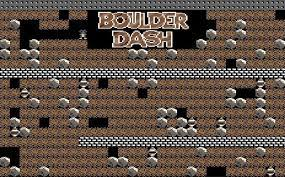
\includegraphics[scale=1.15]{boulder dash.jpeg}~\\[1.5cm]



  \end{center}
  \end{sffamily}
\end{titlepage}


\tableofcontents
\newpage

\section{Descriptif du projet}
\vspace{0.5cm}
\doublebox{
\begin{minipage}{15cm}
Boulder Dash est un jeu où l'on incarne un petit personnage dont le but est de ramasser des diamants en creusant la terre. 
Ce jeu possède différents niveaux dont la difficulté est progressive. Dans ces niveaux, on retrouve des ennemis et des rochers. 
\\Le joueur possède 3 vies, si le joueur se fait écraser par un rocher ou toucher par un ennemi il perd une vie, au bout de 3 vies perdues la partie du joueur est terminée. Certains niveaux ne possèdent pas de diamants, le joueur doit alors tuer les ennemis du niveau en faisant tomber un rocher sur eux ce qui fera apparaître des diamants. Les diamants peuvent aussi tomber sur d'autres ennemis les tuant à leur tour. Le joueur peut aussi casser des murs pour atteindre des zones bloquées grâce aux rochers.
\\Nous avons aussi la volonté d’ajouter des fonctionnalités facultatives telles que la création de niveau par l’utilisateur ou encore la personnalisation du personnage jouable (ces fonctionnalités sont listées dans la partie suivante).
\end{minipage}}
\vspace{1cm}

\section{Fonctionnalités}
\vspace{0.5cm}

\subsection{Fonctionnalités attendues obligatoires}
\begin{itemize}
\item Déplacement du joueur 
\item Chargement des niveaux (mur, terre, bords, rochers) depuis un fichier .txt
\item Sauvegarde de la partie 
\item Différents niveaux
\item Menu
\item Victoire (débloquer passage pour terminer niveau)
\item Détection de mort (écrasé par un rocher, touché par un ennemi) 
\end{itemize}


\subsection{Fonctionnalités facultatives}
\begin{itemize}
    \item Création de niveaux par l’utilisateur
    \item Musique 
    \item Personnalisation joueur
    \item Ajout d’ennemi  et/ou de PNJ
    \item Choix mondes
    \item Chronomètre 
    \item Animation mort personnage (si écrasé par un rocher ou touché par un ennemi)
\end{itemize}

\vspace{0.5cm}
\section{Versions prévues}
\vspace{0.5cm}


\subsubsection*{3.1 Version n°1, date prévue : 08/04/2021}
\vspace{0.2cm}
\addcontentsline{toc}{subsection}{3.1 \hspace{0.1cm} Version n°1, date prévue : 08/04/2021}
\begin{enumerate}[label=]
\item \textit{Fonctionnalités implémentées :} 
\vspace{0.2cm}
   \begin{itemize}
       \item Finalisation des fonctionnalités présentes
       \item Implémentation des fonctionnalités facultatives
   \end{itemize}
   \end{enumerate}
   
\subsubsection*{3.2 Version n°2, date prévue : 22/04/2021}
\vspace{0.2cm}
\addcontentsline{toc}{subsection}{3.2 \hspace{0.1cm} Version n°2, date prévue : 22/04/2021}
\begin{enumerate}[label=]
\item \textit{Fonctionnalités implémentées :} 
\vspace{0.2cm}
   \begin{itemize}
       \item Mise en place de différents niveaux
       \item Sauvegarde de la partie
       \item Implémentation du menu
   \end{itemize}
   \end{enumerate}

\subsubsection*{3.3 Version n°3, date prévue : 07/06/2021}
\vspace{0.2cm}
\addcontentsline{toc}{subsection}{3.3 \hspace{0.1cm} Version n°3, date prévue : 07/06/2021}
\begin{enumerate}[label=]
\item \textit{Fonctionnalités implémentées :} 
\vspace{0.2cm}
\begin{itemize}
       \item Finalisation des fonctionnalités présentes
       \item Implémentation des fonctionnalités facultatives
   \end{itemize}
\end{enumerate}


\end{document}
